\documentclass{beamer}

\usepackage[absolute,overlay]{textpos}
\usepackage{booktabs}
\usepackage{longtable}
\usepackage{amsmath}
\usepackage{color}
\usepackage{empheq}
\usepackage[many]{tcolorbox}
\usepackage[absolute,overlay]{textpos}

\usetheme{Frankfurt}
\usecolortheme{dove}

\definecolor{grey}{gray}{0.45}

\usefonttheme[onlymath]{serif}

% This is to avoid the spaces around \left( and \right)
\let\originalleft\left
\let\originalright\right
\renewcommand{\left}{\mathopen{}\mathclose\bgroup\originalleft}
\renewcommand{\right}{\aftergroup\egroup\originalright}

\newtcbox{\mybox}[1][]{nobeforeafter, math upper, tcbox raise base,
  enhanced, frame hidden, boxrule=0pt, drop lifted shadow, #1}


\title{\bf \color{white} The role of carbon allocation efficiency \\ in the
temperature dependence \\ of growth rates in autotrophs}

\author{\color{white} Bernardo Garc{\'i}a-Carreras \\[3pt] 
  \textrm{\textit \&} \\[3pt]
  {\scriptsize Samraat Pawar, Sof{\'i}a Sal, Dimitrios - Georgios Kontopoulos,\\
    Daniel Padfield, Elvire Bestion, Elisa Schaum, Gabriel Yvon-Durocher}}

\date{\color{white} 18 January 2018\\[5pt]
Silwood Park}


\begin{document}

\setbeamertemplate{itemize item}[square]
\setbeamertemplate{section in toc}[square]
\setbeamerfont{frametitle}{shape=\itshape, series=\bfseries, family=\rmfamily}


{
  \usebackgroundtemplate{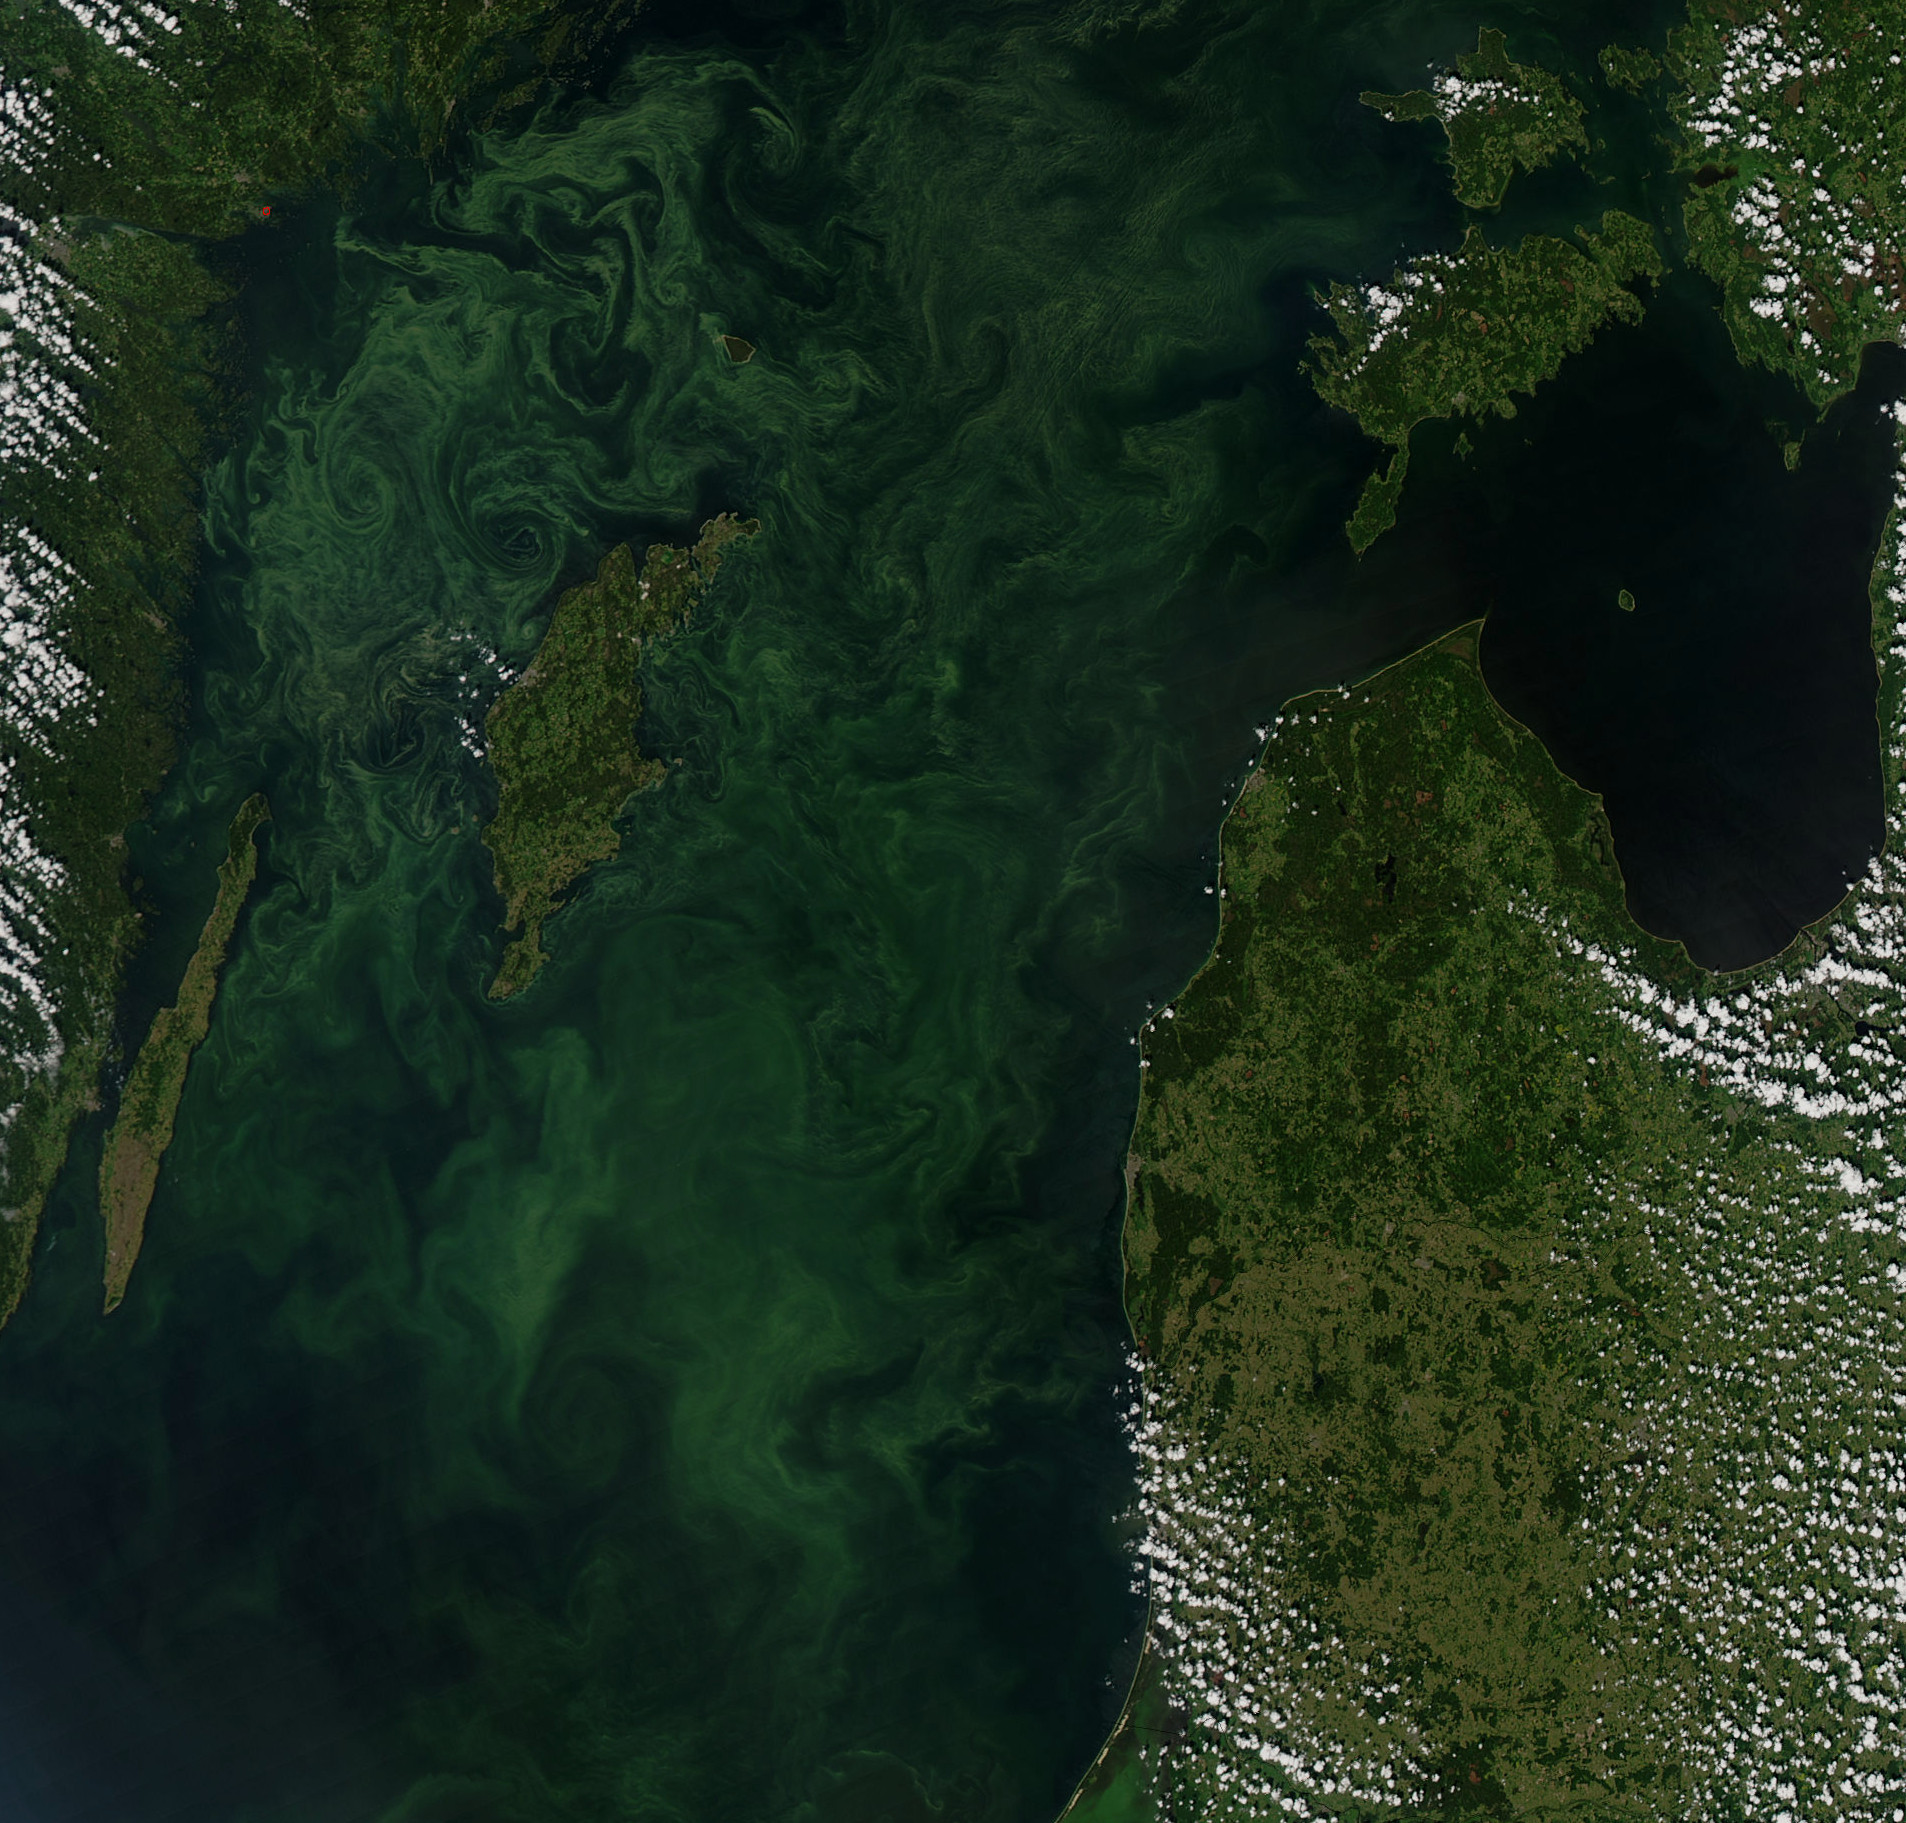
\includegraphics[width=\paperwidth]{figs/algal_bloom2.jpg}}
  \begin{frame}[plain]
    \titlepage

    \begin{textblock*}{13cm}(4mm,91mm)%
      {\tiny \color{white} \textit{Source}: NASA}
    \end{textblock*}
  \end{frame}
}





\section{Introduction}

\subsection{introduction}
\begin{frame}
  \frametitle{Introduction}

  \vspace{-20pt}

  \begin{columns}
    \begin{column}{0.65\textwidth}
      \begin{itemize}
        \item Autotroph population growth rates are temperature dependent.
        \item Patterns in weather and climate are changing.
        \item We need a more mechanistic understanding of growth rate thermal
          performance curves (TPCs).
        \item Key metabolic rates include photosynthesis, respiration\ldots
        \item But what about {\textrm{\textit{efficiency?}}}
      \end{itemize}
    \end{column}
    \begin{column}{0.48\textwidth}
    \end{column}
  \end{columns}

  \begin{textblock*}{4.5cm}(0.77\textwidth,7mm)%
    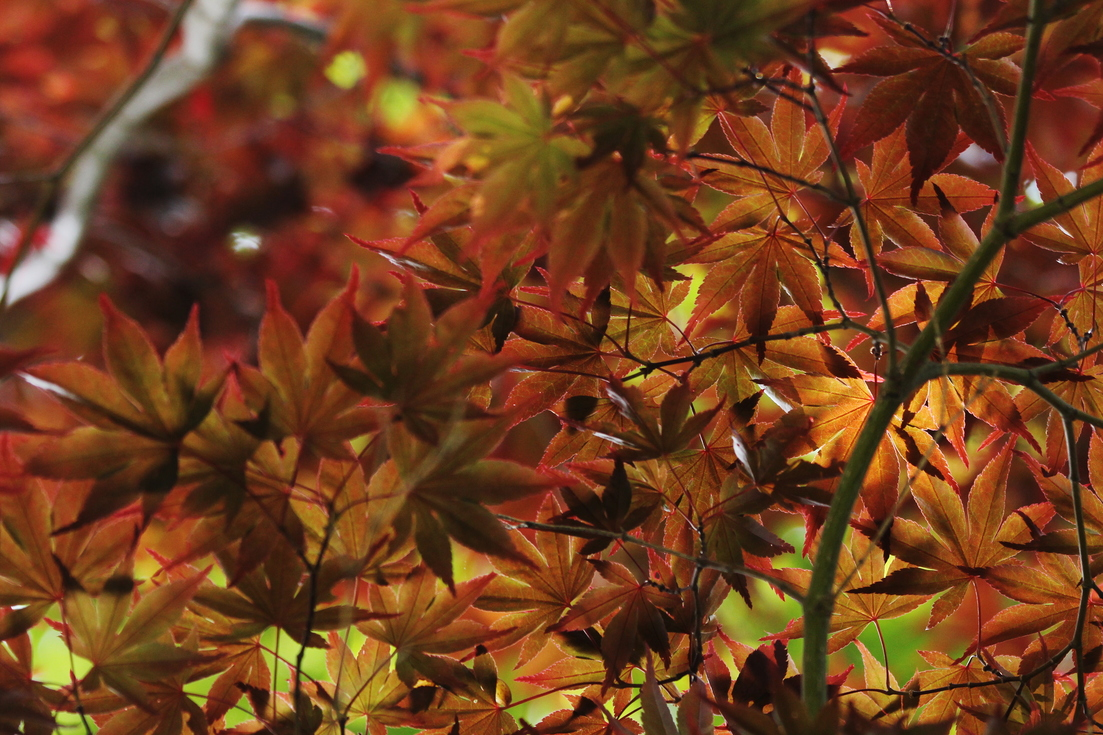
\includegraphics[width=\textwidth]{figs/random/leaves1.jpg}\\[-2pt]
    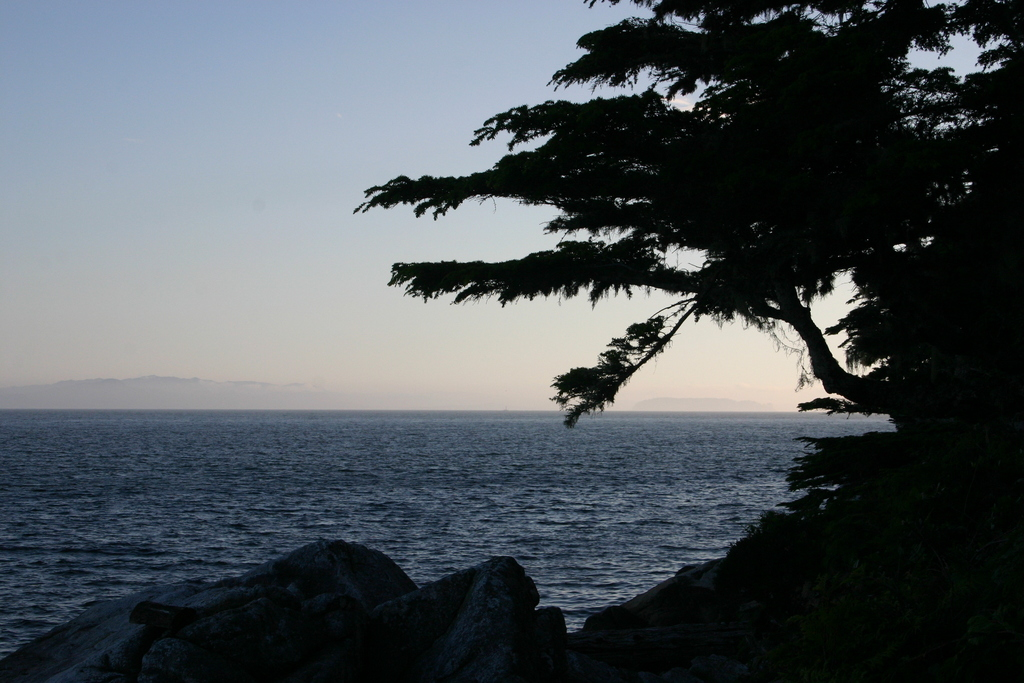
\includegraphics[width=\textwidth]{figs/random/sea1.jpg}\\[-2pt]
    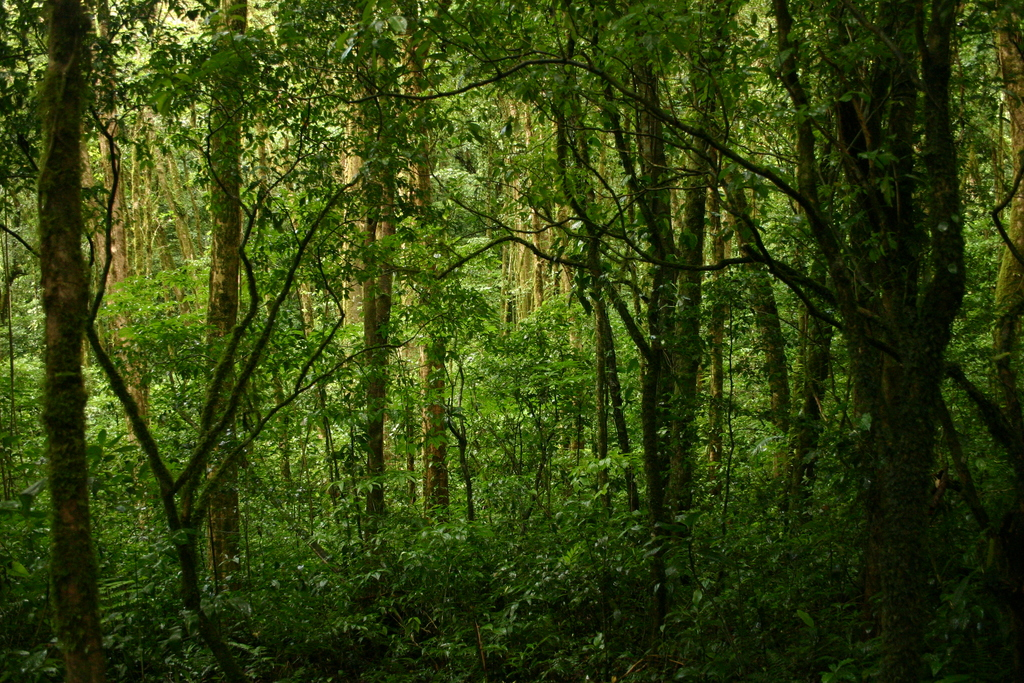
\includegraphics[width=\textwidth]{figs/random/cr1.jpg}
  \end{textblock*}

\end{frame}



\subsection{plan}
\begin{frame}
  \frametitle{Introduction}

  \begin{textblock*}{4.2cm}(0mm,13mm)%
    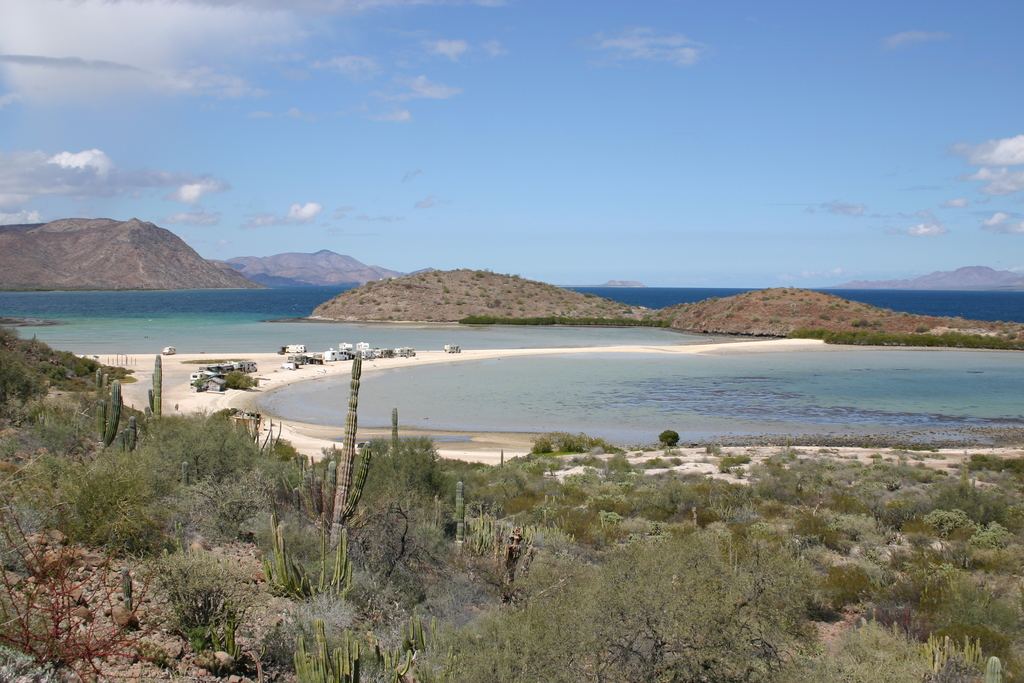
\includegraphics[width=\textwidth]{figs/random/desert5.jpg}\\[-2pt]
    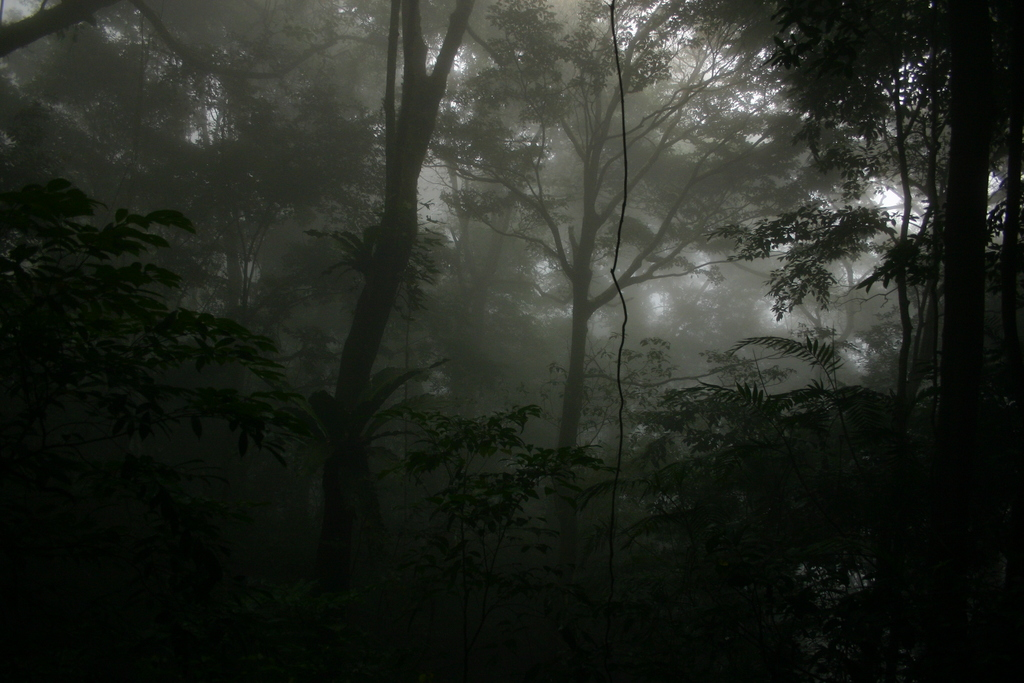
\includegraphics[width=\textwidth]{figs/random/cr2.jpg}\\[-2pt]
    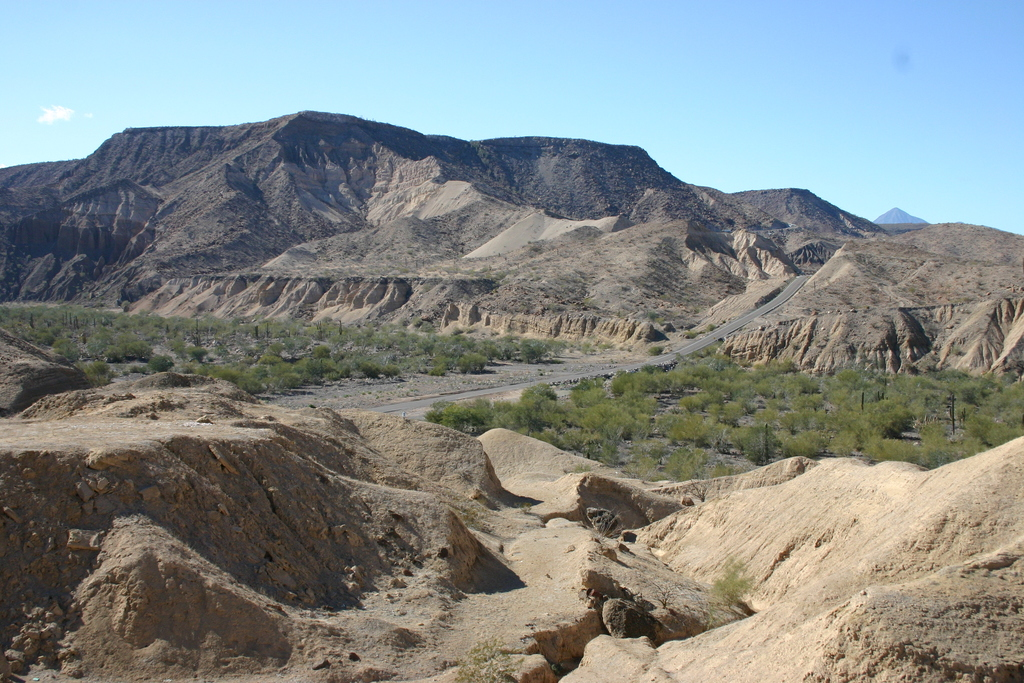
\includegraphics[width=\textwidth]{figs/random/desert2.jpg}
  \end{textblock*}

  \begin{columns}
    \begin{column}{0.40\textwidth}
    \end{column}
    \begin{column}{0.75\textwidth}
      I will:
      \begin{itemize}
        \item Introduce the population model.
        \item Fit it to data from a unique laboratory experiment on a
          phytoplankton species.
        \item Explore the potential importance of temperature-dependent
          allocation efficiency across a wider range of species using a
          meta-analysis.
      \end{itemize}
    \end{column}
  \end{columns}

\end{frame}





\section{Theory}

\subsection{theory1}
\begin{frame}
  \frametitle{The model}

  \begin{empheq}[box=\mybox]{equation*}
    \frac{1}{N} \, \frac{\mathrm{d} N}{\mathrm{d} t} = r = \varepsilon \, F
  \end{empheq}
  where
  \begin{itemize}
    \item $N$ is the autotroph population's biomass density.\\
    \item $r$ is the growth rate.\\
    \item Net carbon flux $F = P - R$.\\
    \item $\varepsilon$ is carbon allocation efficiency.
  \end{itemize}

\end{frame}



\subsection{theory2}
\begin{frame}
  \frametitle{Photosynthesis $P$ \& respiration $R$}

  \begin{empheq}[box=\mybox]{equation*} 
    B = \frac{B_0 \, \exp\left(-\dfrac{E}{k} \, \left(\dfrac{1}{T} -
    \dfrac{1}{T_\mathrm{ref}}\right)\right)}
    {1 + \exp\left(\dfrac{E_\mathrm{D}}{k} \, \left(\dfrac{1}{T_\mathrm{h}} -
    \dfrac{1}{T}\right)\right)}
  \end{empheq}

  \begin{center}
    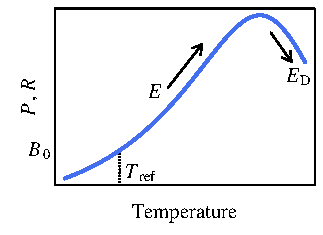
\includegraphics{figs/school.pdf}
  \end{center}
\end{frame}



\subsection{theory3}
\begin{frame}
  \frametitle{Allocation efficiency $\varepsilon$}

  \begin{empheq}[box=\mybox]{equation*} 
    \varepsilon = \varepsilon_0 \, \exp\left(-\frac{E_\varepsilon}{k} \,
    \left(\frac{1}{T} - \frac{1}{T_\mathrm{ref}}\right)\right)
  \end{empheq}

  \begin{center}
    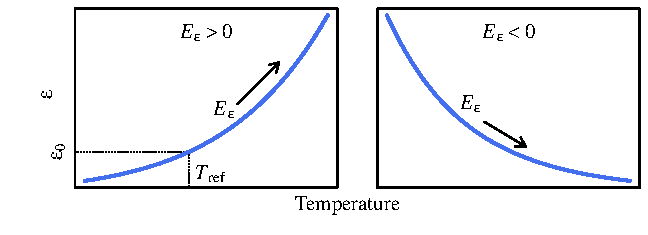
\includegraphics{figs/ba.pdf}
  \end{center}
\end{frame}





\section{An experiment}

\subsection{experiment1}
\begin{frame}
  \frametitle{A laboratory experiment: \textit{Chlorella vulgaris}}

  \vspace{-20pt}
  \begin{center}
    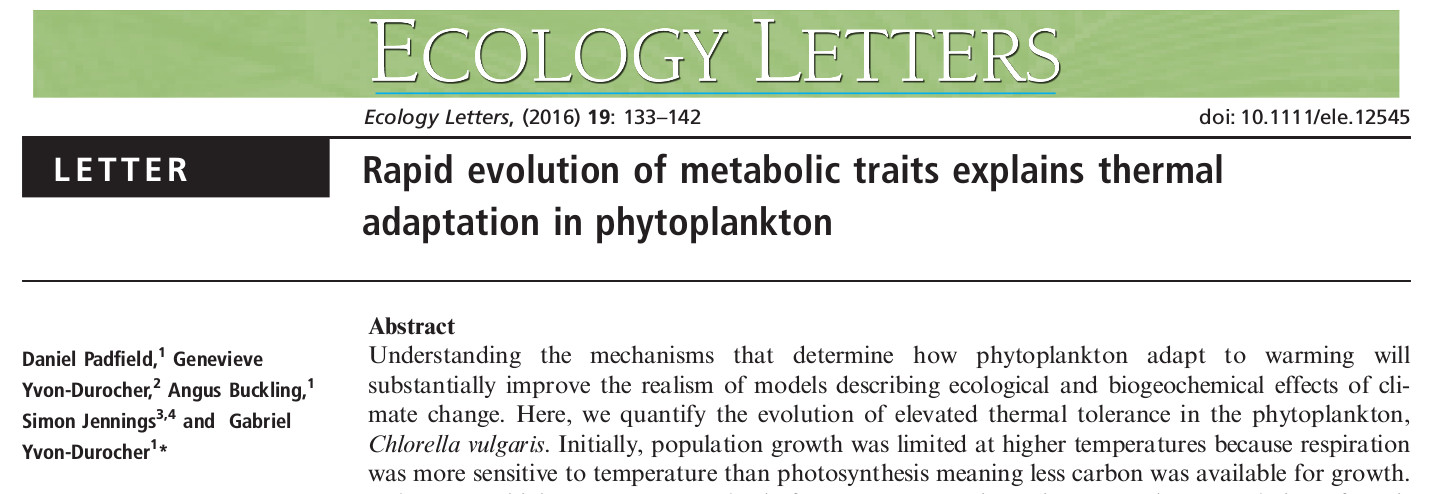
\includegraphics[width=0.8\textwidth]{figs/padfield.jpg}
  \end{center}

  \vspace{7pt}

  \begin{columns}
    \begin{column}{0.55\textwidth}
      Isolated from a pond in N.\ England, maintained at 20$^\circ$C.\\[7pt]

      Growth, $P$ and $R$ for two sets of populations:
      \begin{itemize}
        \item \textit{Acclimated}: $\approx 10$ generations. 
        \item \textit{Adapted}: $\approx 100$ generations. 
      \end{itemize}
    \end{column}
    \begin{column}{0.42\textwidth}
      \begin{center}
        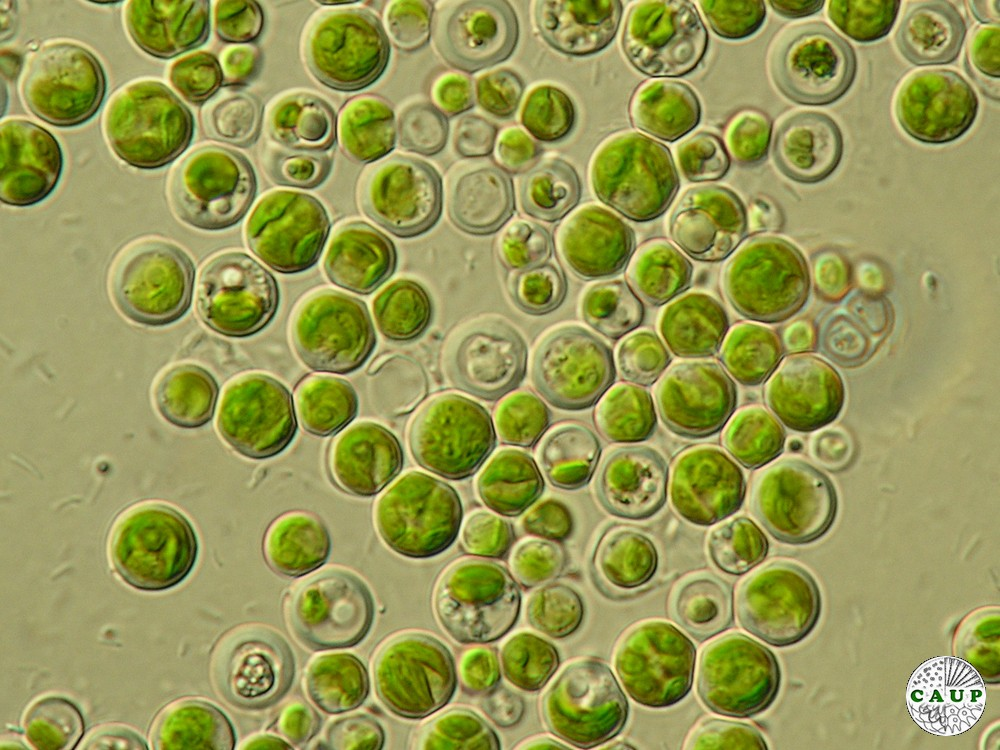
\includegraphics[width=\textwidth]{figs/chlorella.JPG}\\[-8pt]
        {\tiny \textit{Source}: botany.natur.cuni.cz}
      \end{center}
    \end{column}
  \end{columns}

\end{frame}



\subsection{experiment2}
\begin{frame}
  \frametitle{A laboratory experiment: \textit{Chlorella vulgaris}}

  \begin{center}
    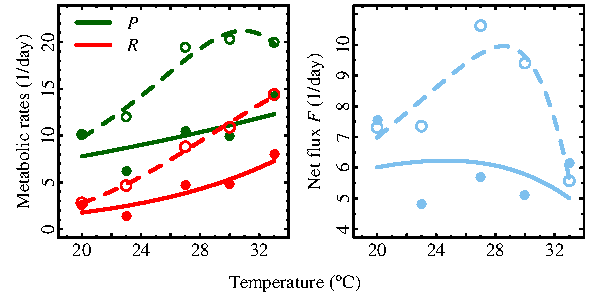
\includegraphics{figs/dan_res_pres.pdf}
  \end{center}

\end{frame}



\subsection{experiment3}
\begin{frame}
  \frametitle{A laboratory experiment: \textit{Chlorella vulgaris}}

  \begin{center}
    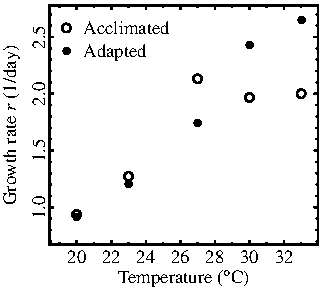
\includegraphics{figs/dan_res3_pres.pdf}
  \end{center}

\end{frame}



\subsection{experiment4}
\begin{frame}
  \frametitle{A laboratory experiment: \textit{Chlorella vulgaris}}

  \begin{center}
    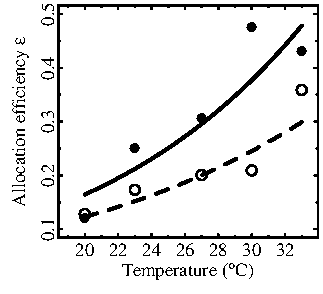
\includegraphics{figs/dan_res_eps_pres.pdf}
  \end{center}

\end{frame}



\subsection{experiment5}
\begin{frame}
  \frametitle{A laboratory experiment: \textit{Chlorella vulgaris}}

  \begin{center}
    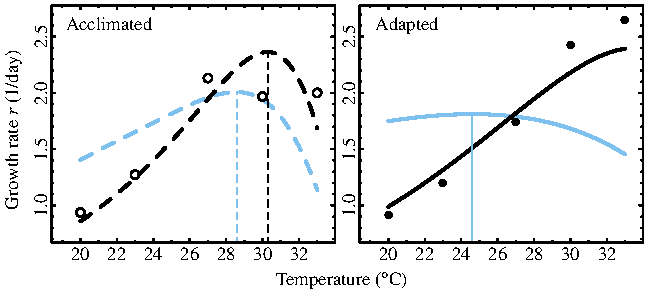
\includegraphics{figs/dan_res2_pres.pdf}
  \end{center}

\end{frame}





\section{A meta-analysis}

\subsection{moss1}
\begin{frame}
  \frametitle{A meta-analysis}

  \vspace{-20pt}

  \begin{center}
    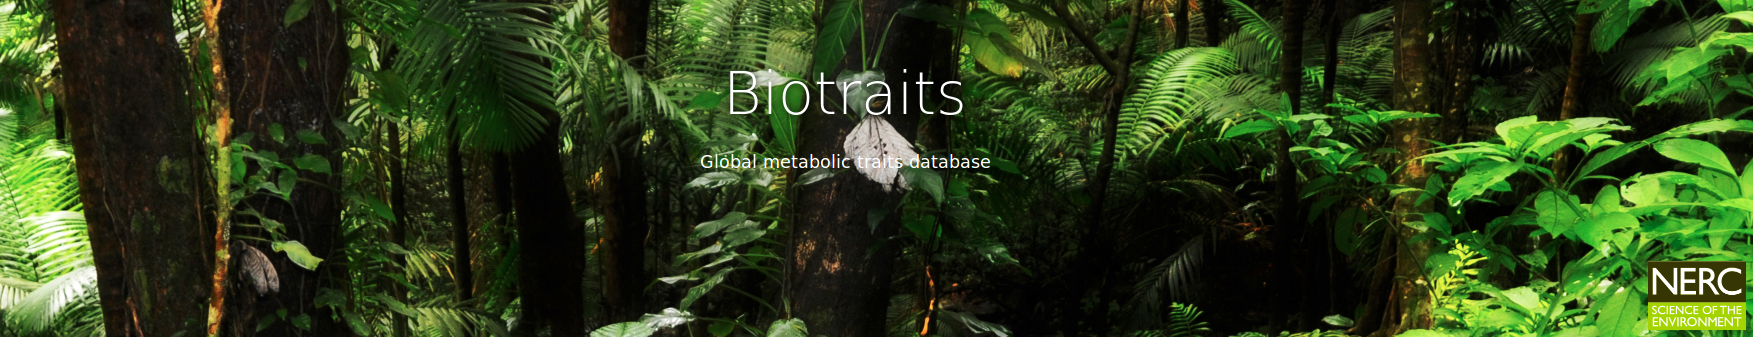
\includegraphics[width=0.9\textwidth]{figs/biotraits.png}
  \end{center}

  \vspace{10pt}

  Extracted autotroph TPCs for which both $P$ and $R$ were measured on the same
  population. Filtering produced:
  \begin{itemize}
    \item 21 pairs of TPCs for aquatic species.
    \item 22 pairs of TPCs for terrestrial species.
    \item 38 species in total. 
  \end{itemize}

\end{frame}



\subsection{moss2}
\begin{frame}
  \frametitle{An example}

  \begin{center}
    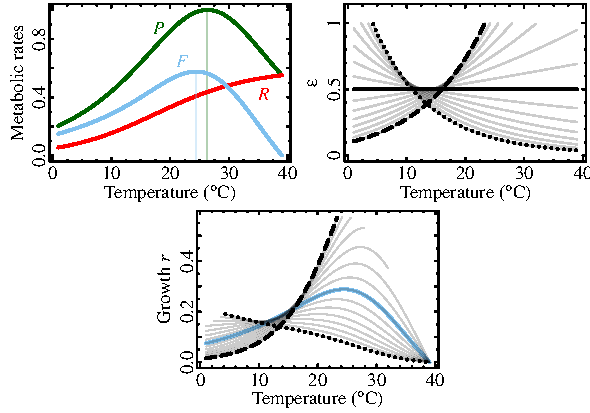
\includegraphics{figs/example_intro_pres.pdf}
  \end{center}
\end{frame}



\subsection{moss3}
\begin{frame}
  \frametitle{An example}

  \begin{center}
    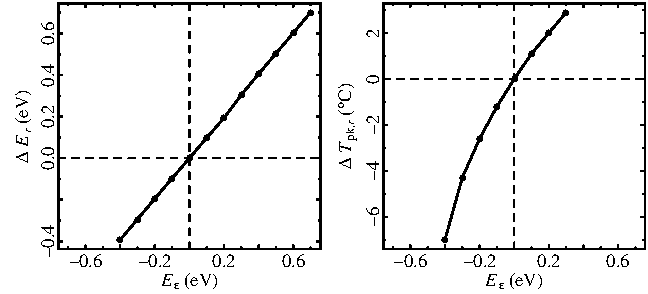
\includegraphics{figs/example_intro_pres2.pdf}
  \end{center}
\end{frame}



\subsection{ma1}
\begin{frame}
  \frametitle{A meta-analysis}

  \begin{center}
    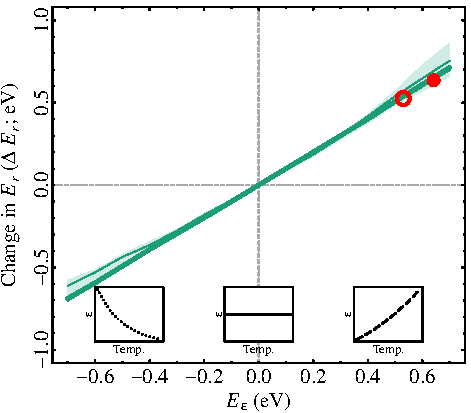
\includegraphics{figs/sofia_pres1.pdf}
  \end{center}
\end{frame}



\subsection{ma2}
\begin{frame}
  \frametitle{A meta-analysis}

  \begin{center}
    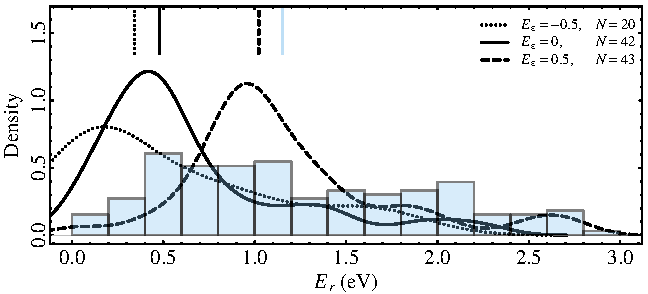
\includegraphics{figs/sofia_pres2.pdf}
  \end{center}
\end{frame}



\subsection{ma3}
\begin{frame}
  \frametitle{A meta-analysis}

  \begin{center}
    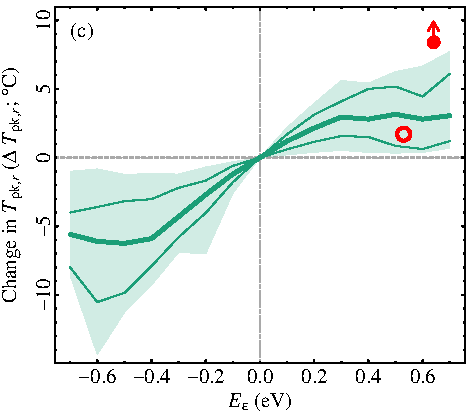
\includegraphics{figs/sofia_pres3.pdf}
  \end{center}
\end{frame}



\subsection{ma4}
\begin{frame}
  \frametitle{A meta-analysis}

  \begin{center}
    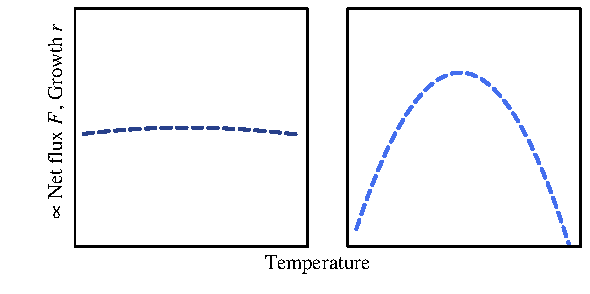
\includegraphics{figs/delta_tpk_ex.pdf}
  \end{center}
\end{frame}



\subsection{ma5}
\begin{frame}
  \frametitle{A meta-analysis}

  \begin{center}
    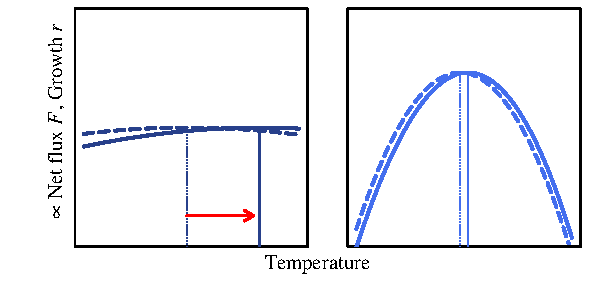
\includegraphics{figs/delta_tpk_ex2.pdf}
  \end{center}
\end{frame}





\section{Discussion}

\subsection{nutrients}
\begin{frame}
  \frametitle{Nutrient limitation}

  \begin{empheq}[box=\mybox]{align*}
    r &= \varepsilon \, F \, {\color{red} V}, \quad \text{with} \\[5pt]
    V &= \frac{S}{K_S + S}
  \end{empheq}

  \begin{columns}
    \begin{column}{0.48\textwidth}
      \begin{center}
        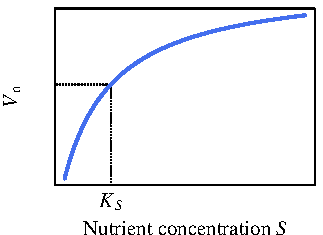
\includegraphics{figs/nuts.pdf}
      \end{center}
    \end{column}
    \begin{column}{0.48\textwidth}
      If $K_S$ increases with $T$, \\ $V$ decreases with $T$, and
      \begin{itemize}
        \item $E_r$ is reduced, and
        \item $T_{\mathrm{pk},r}$ is reduced,
      \end{itemize}
      analogous to when $E_\varepsilon < 0$.
    \end{column}
  \end{columns}

\end{frame}



\subsection{respiration}
\begin{frame}
  \frametitle{Respiration}

  \begin{empheq}[box=\mybox]{equation*}
    \frac{1}{N} \, \frac{\mathrm{d} N}{\mathrm{d} t} = r = \varepsilon \, 
    (P - {\color{red}{R}})
  \end{empheq}

  \begin{itemize}
    \item Role of respiration greatly simplified.
    \item $R$ uses carbon, making it unavailable for growth\ldots
    \item \ldots but $R$ also supports growth (e.g., ATP production).
    \item Disentangle what components of respiration are measured in $P$ and $R$
      in experiments.
  \end{itemize}
\end{frame}



\subsection{heterotrophs}
\begin{frame}
  \frametitle{Heterotrophs}

  \begin{itemize}
    \item Implications of temperature-dependence in $\varepsilon$ extend to
      heterotrophs, e.g., mass-conversion efficiency.
    \item Variation in growth rate TPCs might stem from variation in
      $\varepsilon$.
    \item Growth and metabolism not necessarily interchangeable. 
  \end{itemize}
  
  \begin{center}
    \hspace{20pt} 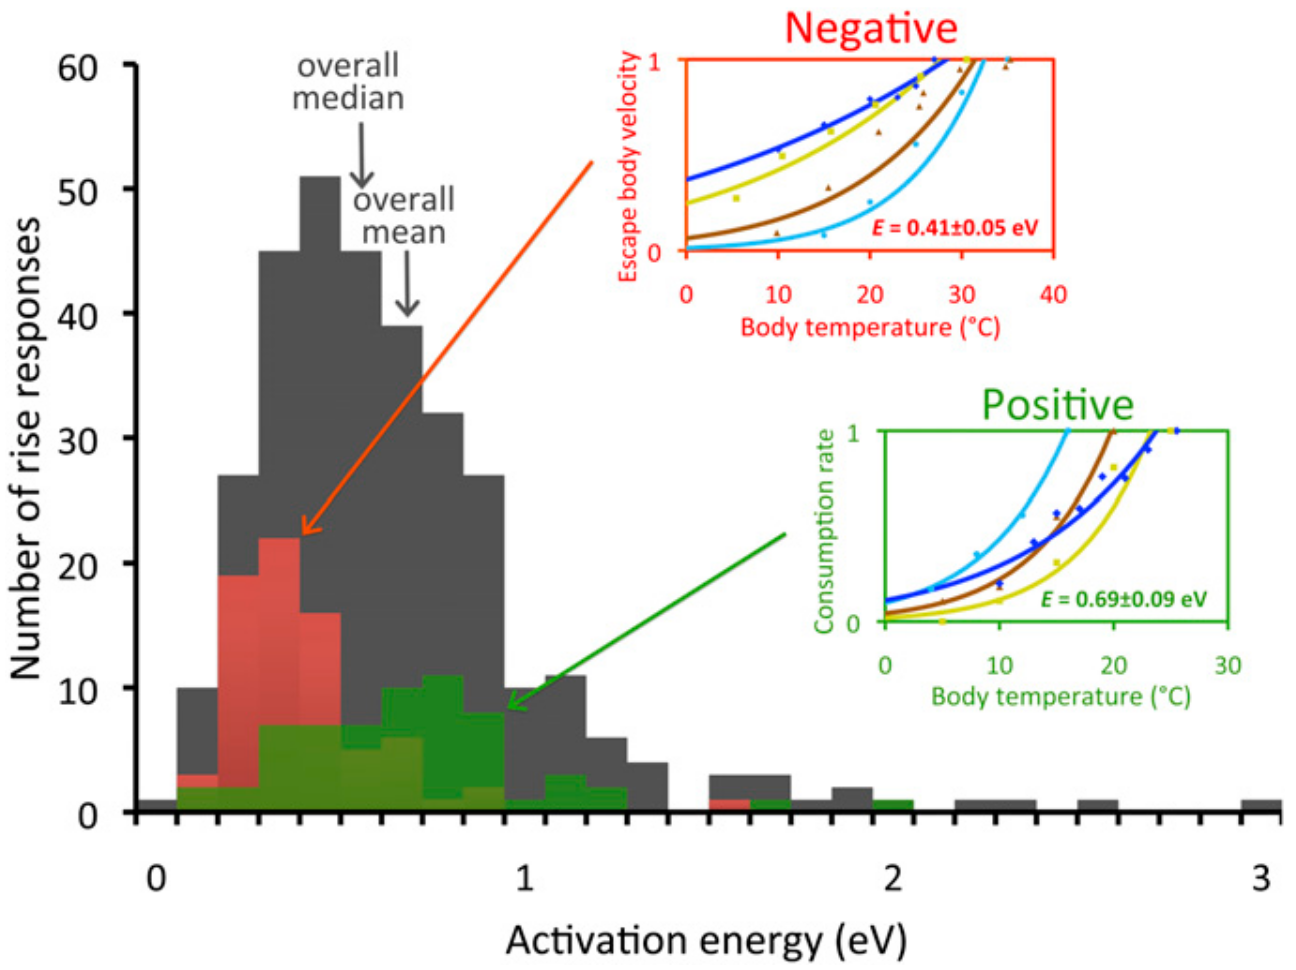
\includegraphics[width=0.6\textwidth]{figs/delletal.png}
  \end{center}

  \vspace{-15pt}
  {\tiny  \hspace{10pt} \textit{Source}: Dell, Pawar \& Savage (2011). \textit{PNAS}.}
\end{frame}



\subsection{data}
\begin{frame}
  \frametitle{Experiments}

  \vspace{-2cm}
  We recommend further experiments!
  \begin{itemize}
    \item Growth, $P$, $R$, at the same levels of acclimation / adaptation to
      temperature.
    \item Preferably measuring metabolic rates on the \textit{same} cells
      undergoing growth.
    \item A reasonable number of replicates.
    \item Across a range of species.
  \end{itemize}

  These would allow us to quantify variation in $\varepsilon$.
  
  \begin{textblock*}{4.3cm}(0mm,68mm)%
    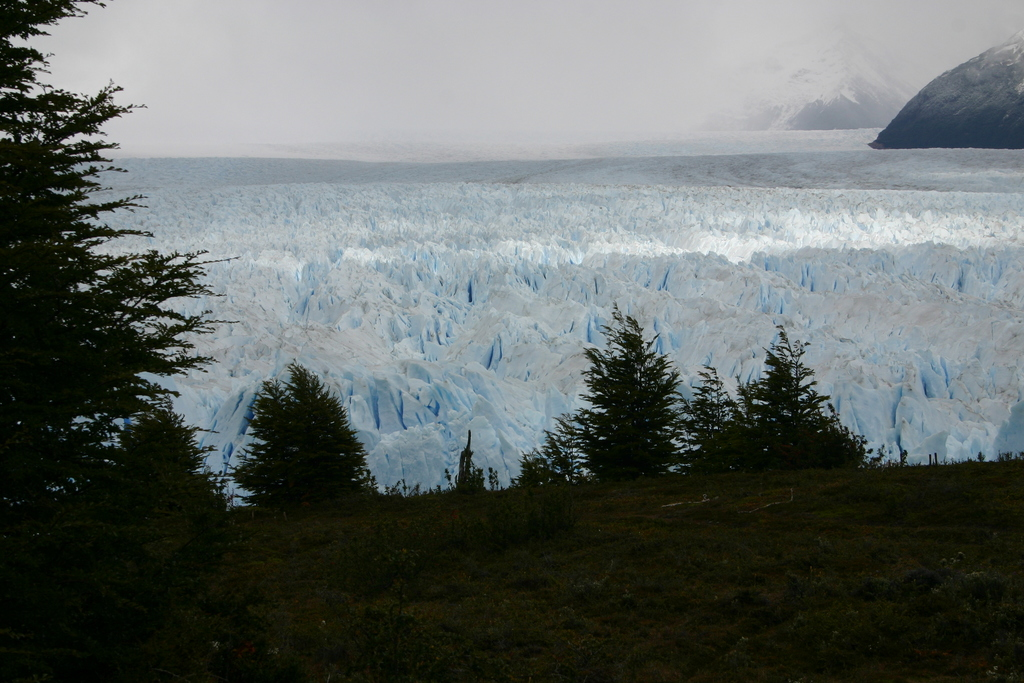
\includegraphics[width=\textwidth]{figs/random/sea3.jpg}
    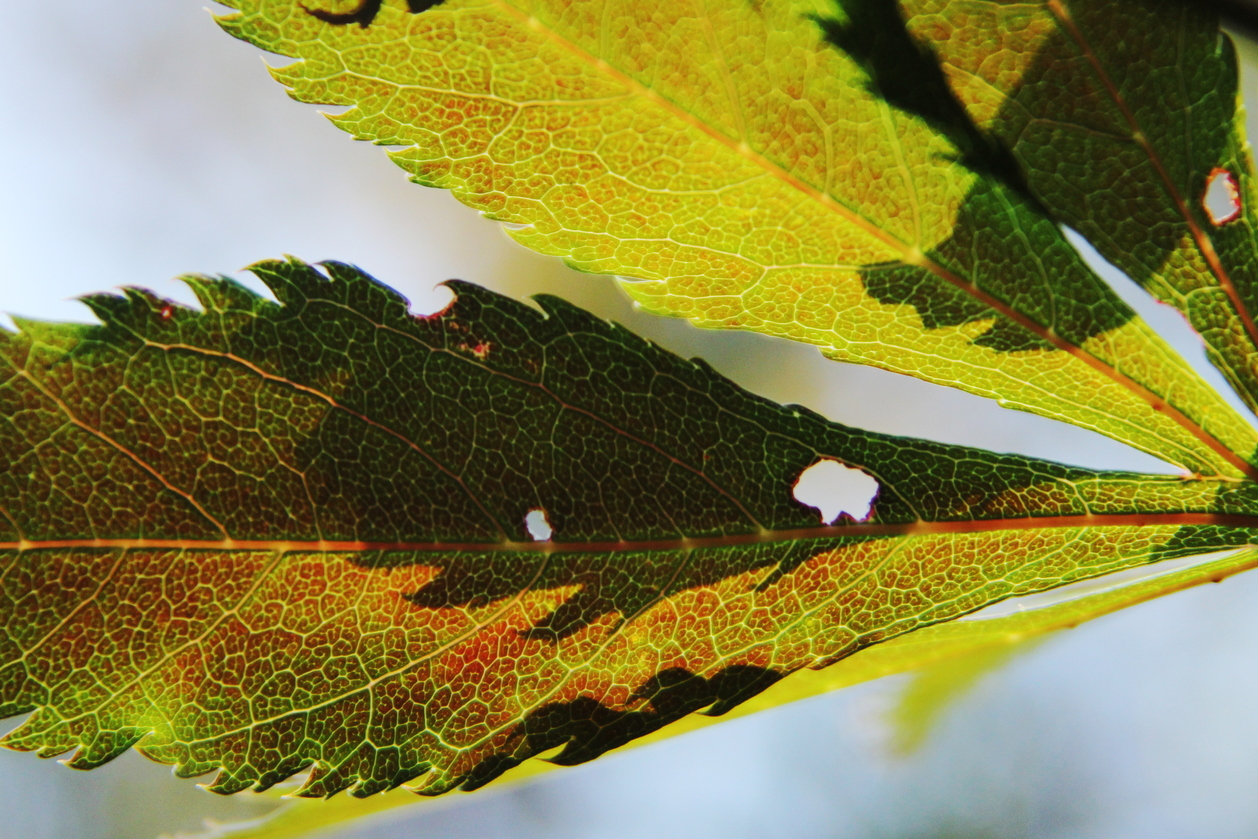
\includegraphics[width=\textwidth]{figs/random/leaves3.jpg}
    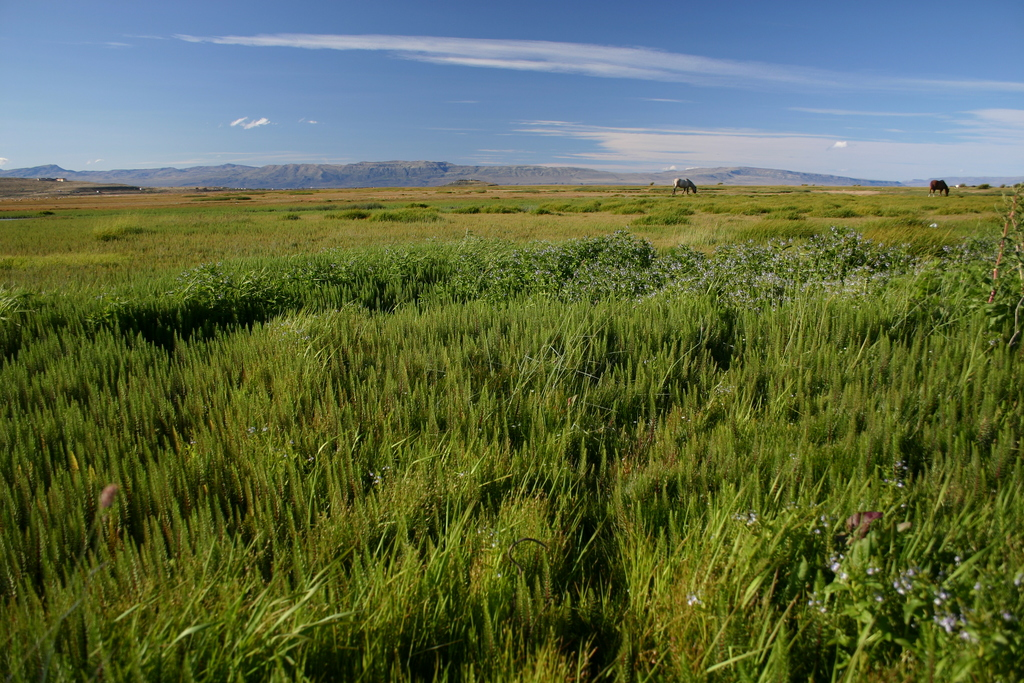
\includegraphics[width=\textwidth]{figs/random/arg1.jpg}
  \end{textblock*}
\end{frame}



\subsection{conclusion}
\begin{frame}
  \frametitle{Conclusion}

  \begin{textblock*}{4.5cm}(0.77\textwidth,7mm)%
    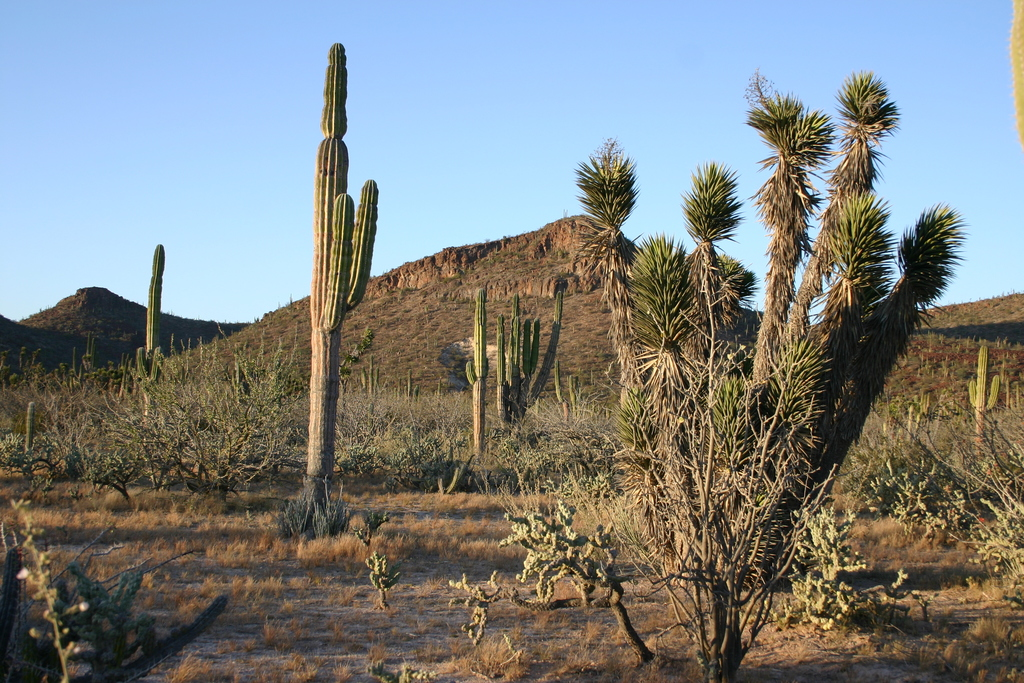
\includegraphics[width=\textwidth]{figs/random/desert1.jpg}\\[-2pt]
    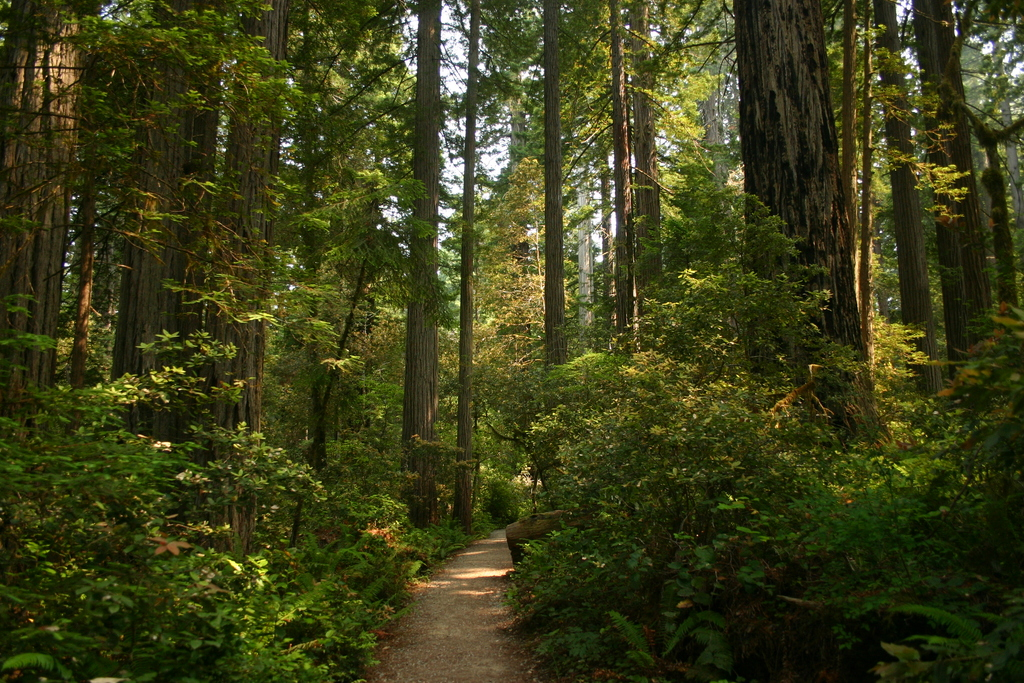
\includegraphics[width=\textwidth]{figs/random/forest1.jpg}\\[-2pt]
    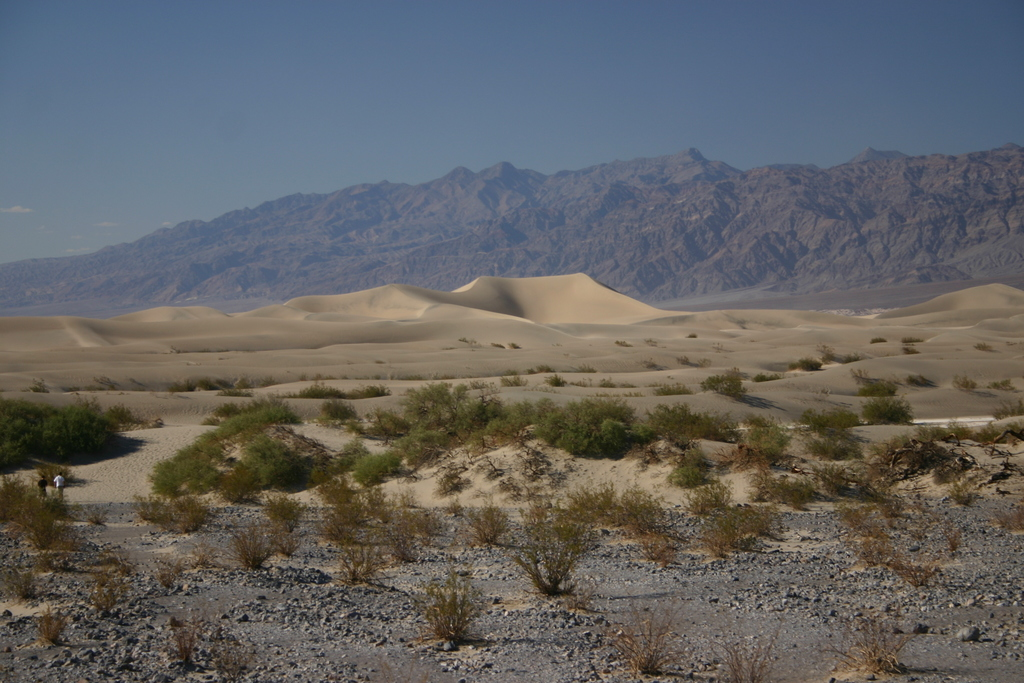
\includegraphics[width=\textwidth]{figs/random/desert4.jpg}
  \end{textblock*}

  \begin{columns}
    \begin{column}{0.65\textwidth}
      \begin{itemize}
        \item A simple framework that only requires measurement of three rates
          (growth, $P$, $R$) to better understand the temperature dependence of
          growth. 
        \item Necessary step prior to developing more mechanistic models.
        \item Demonstrated the potential importance of temperature dependence of
          allocation efficiency.
      \end{itemize}
    \end{column}
    \begin{column}{0.4\textwidth}
    \end{column}
  \end{columns}

\end{frame}



\subsection{thanks}
\begin{frame}[plain]
  \frametitle{}

  \begin{textblock*}{13cm}(0mm,0mm)%
    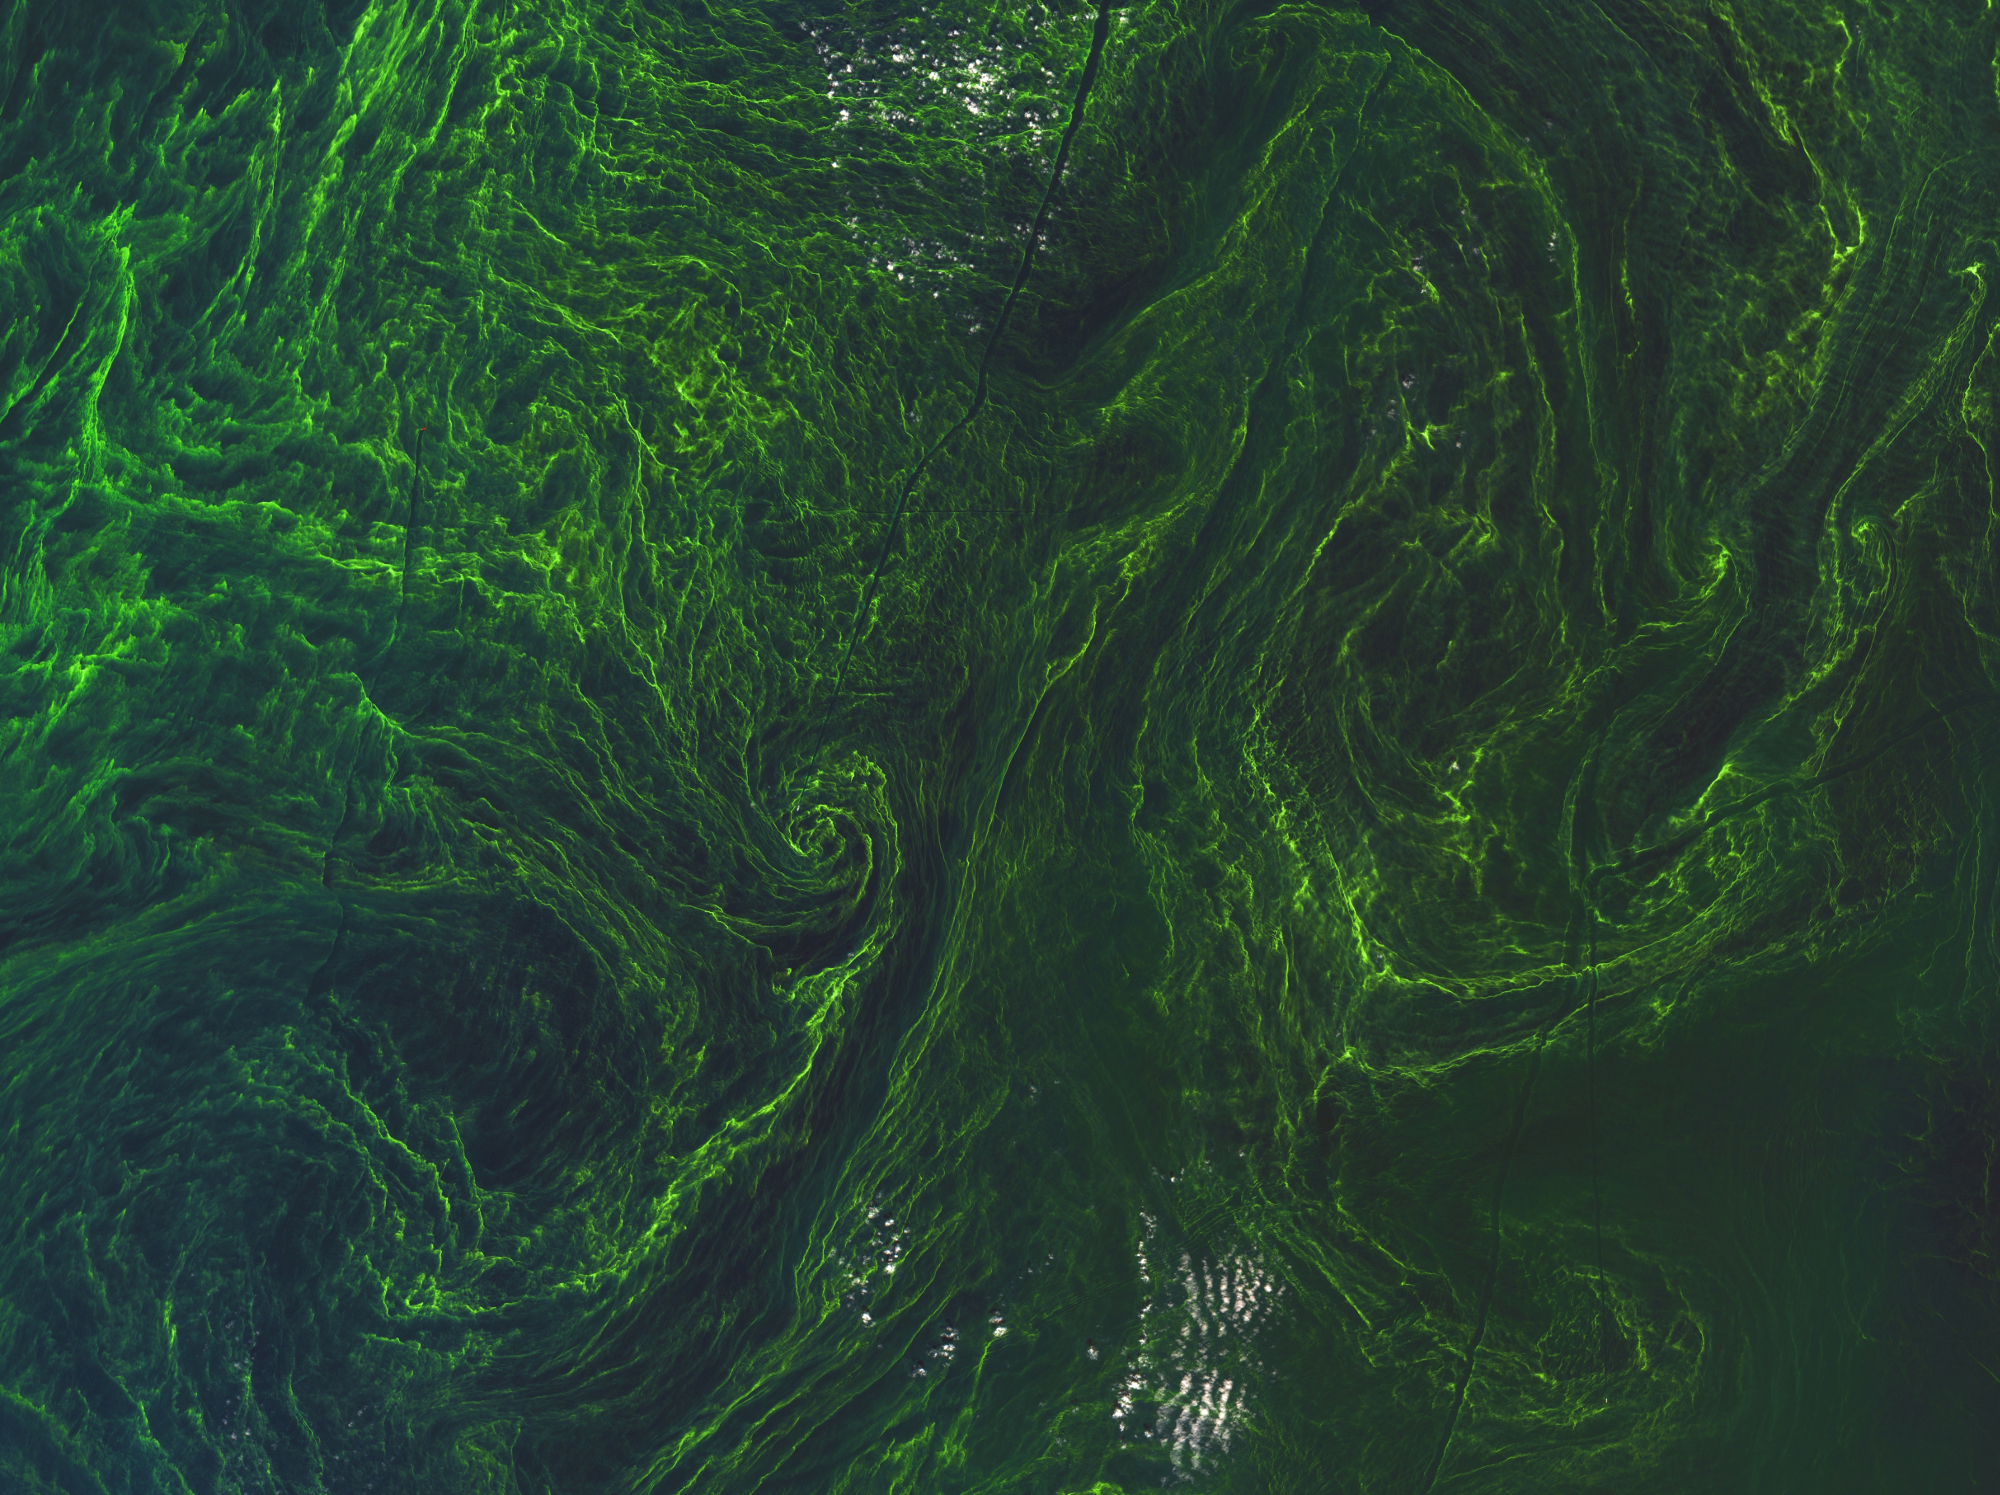
\includegraphics[width=\textwidth]{figs/Algae_storm2.jpg}
  \end{textblock*}

  \begin{textblock*}{13cm}(0mm,40mm)%
    \begin{center}
      {\Huge \bf \color{white} Thank you!}
    \end{center}
  \end{textblock*}

  \begin{textblock*}{13cm}(0mm,82mm)%
    \begin{center}
      {\Large \color{white} bgarciacarreras@gmail.com}
    \end{center}
  \end{textblock*}

  \begin{textblock*}{13cm}(0mm,82mm)%
    \begin{center}
      {\Large \color{white} bgarciacarreras@gmail.com}
    \end{center}
  \end{textblock*}

  \begin{textblock*}{13cm}(4mm,91mm)%
    {\tiny \color{white} \textit{Source}: ESA}
  \end{textblock*}
\end{frame}



\end{document}

